\documentclass[12pt]{extarticle}

%Some packages I commonly use.
\usepackage[english]{babel}
\usepackage{graphicx}
\usepackage{framed}
\usepackage[normalem]{ulem}
\usepackage{amsmath}
\usepackage{amsthm}
\usepackage{amssymb}
\usepackage{amsfonts}
\usepackage{enumerate}
\usepackage[utf8]{inputenc}
\usepackage{float}
\usepackage{gensymb}
\usepackage[top=1 in,bottom=1in, left=1 in, right=1 in]{geometry}
\usepackage{multirow}
\usepackage{caption}
\usepackage{subcaption}
\usepackage[utf8]{inputenc}

%A bunch of definitions that make my life easier
\newcommand{\matlab}{{\sc Matlab} }
\newcommand{\cvec}[1]{{\mathbf #1}}
\newcommand{\rvec}[1]{\vec{\mathbf #1}}
\newcommand{\ihat}{\hat{\textbf{\i}}}
\newcommand{\jhat}{\hat{\textbf{\j}}}
\newcommand{\khat}{\hat{\textbf{k}}}
\newcommand{\minor}{{\rm minor}}
\newcommand{\trace}{{\rm trace}}
\newcommand{\spn}{{\rm Span}}
\newcommand{\rem}{{\rm rem}}
\newcommand{\ran}{{\rm range}}
\newcommand{\range}{{\rm range}}
\newcommand{\mdiv}{{\rm div}}
\newcommand{\proj}{{\rm proj}}
\newcommand{\R}{\mathbb{R}}
\newcommand{\N}{\mathbb{N}}
\newcommand{\Q}{\mathbb{Q}}
\newcommand{\Z}{\mathbb{Z}}
\newcommand{\<}{\langle}
\renewcommand{\>}{\rangle}
\renewcommand{\emptyset}{\varnothing}
\newcommand{\attn}[1]{\textbf{#1}}
\theoremstyle{definition}
\newtheorem{theorem}{Theorem}
\newtheorem{corollary}{Corollary}
\newtheorem*{definition}{Definition}
\newtheorem*{example}{Example}
\newtheorem*{note}{Note}
\newtheorem{exercise}{Exercise}
\newcommand{\bproof}{\bigskip {\bf Proof. }}
\newcommand{\eproof}{\hfill\qedsymbol}
\newcommand{\Disp}{\displaystyle}
\newcommand{\qe}{\hfill\(\bigtriangledown\)}
\setlength{\columnseprule}{1 pt}
\usepackage[utf8]{inputenc}

\title{Gases - Lei Geral e transformações}
\author{Felipe Salvador}
\date{Outubro 2019}

\begin{document}

\maketitle

\section*{Introdução}
    
    Nessa parte da matéria de Termodinâmica, veremos como gases se comportam, como grandezas físicas que podemos medir, como volume e temperatura, se comportam quando estamos falando de gases. Iremos enunciar um equação importante, chamada de Lei Geral dos Gases
    
    Além disso, iremos algumas transformações especiais que gases podem fazer e descrever relações para cada transformação. Por fim, analisaremos como cada transformação ocorre por meio de gráficos.
    
    
\section{Gases - Modelo dos Gases Ideais.}
    
    Gás é um estado da matéria que ocorre quando a distância entre 2 moléculas/átomos é bem grande, de forma que a interação entre eles é bem pequena. Um gás, assim como um líquido, não tem forma definida, a forma irá depender do compartimento que estiver contendo o gás. 
    
    O que difere de um gás de um líquido é a interação entre átomos/moléculas. No líquido, as moléculas interagem umas com as outras tão intensamente que as moléculas ainda ficam juntas, elas não se dispersam. Isso é diferente para um gás, pois a atração entre as moléculas é tão fraca, que as moléculas de um gás vão cada uma para um lado. \footnote{Existem exceções, mas são casos de um gás feito de, pelo menos 1, substância muito eletronegativa. Um exemplo disso é o gás cloro ($Cl_2$)}
    
    Então, nós iremos tratar gases da forma mais simples possível. Não nos preocuparemos com atração/repulsão entre moléculas, geometria da molécula/átomo (formato), nem de uma possível liquefação (quando gás se transforma em líquido). Para essas suposições, construímos um modelo chamado de \textbf{Gases Ideais}.
    
    Nesse modelo, tomamos as seguintes suposições:
    \begin{itemize}
        \item As moléculas/átomos não interagem entre si;
        \item O formato das moléculas é esférico (bola);
        \item Qualquer colisão entre uma molécula/átomo com a parede da garrafa ou com outra molécula é uma colisão elástica (não perde energia e não gruda com a parede ou molécula);
        \item Posso comprimir, aquecer, esfriar, expandir o quanto eu quiser que ainda será um gás.
    \end{itemize}
    
    Com isso, temos um modelo de gás fundamental inicial. Ele descreve bem os gases quando esses gases são rarefeitos (poucas moléculas por volume), estão a uma temperatura muito altas e/ou são gases nobres (como o Hélio ($He$) e o Neônio($Ne$)).
    
    Nesse modelo, temos uma equação a qual damos o nome de \textbf{Lei Geral dos Gases Ideais}:
    
    \begin{equation}\label{eq:Lei}
        P V = n R T
    \end{equation}
em que $P$ é a pressão do gás, $V$ é o volume que o gás ocupa, $n$ é o número de mols do gás no recipiente e $T$ é a temperatura do gás.

Só faltou descrever $R$. Isso é a \textbf{Constante Universal dos Gases Ideais}. Ela é um número, que depende das unidades que eu usar para a pressão, temperatura e volume.

Nas unidades mais usuais, a pressão é \textbf{Atmosfera (atm)}, o volume é \textbf{Litro (L)} e temperatura é \textbf{Kelvin (K)}. Nessas unidades, $R$ é:
\begin{equation}
    R = 0,082 \:\frac{atm\,L}{mol\,K}
\end{equation}

Outras unidades usuais são: Pressão em mílimetros de Mercúrio (mmHg). Para essa mudança, $R$ é:
\begin{equation}
    R = 62,3 \:\frac{mmHg\,L}{mol\,K}
\end{equation}

Essa equação (\eqref{eq:Lei}) vale para todas as medidas de pressão, volume e temperatura e até mesmo para quando saimos de um estado (com certos valores de temperatura, pressão e volume) para outro estado (com outros valores de temperatura, pressão e volume). Todas as transformações de um estado para outro, nós iremos considerar que não há perda ou ganho de moléculas de gás. Ou seja, \textbf{n é um valor constante}.

Com isso, podemos isolar todas as variáveis que podem mudar para um lado da equação e obtemos:
\begin{equation}
    \frac{PV}{T} = nR = \text{constante}
\end{equation}

Ou seja, dado um gás que esteja num estado inicial que tenha as seguintes medidas $(V_i,P_i,T_i)$ e vá para um estado final que tenha as seguintes medidas $(V_f,P_f,T_f)$, pela última equação, temos que:

\begin{align}
    \frac{P_i V_i}{T_i} &= nR = \text{constante} & \frac{P_f V_f}{T_f} &= nR = \text{constante}
\end{align}

Como os lados direitos são iguais, então:

\begin{equation}
    \frac{P_i V_i}{T_i} = \frac{P_f V_f}{T_f}
\end{equation}

\textbf{Essa última equação damos o nome de Equação de Clapeyron}

Essa equação relaciona as medidas entre o estado inicial e final de um processo. Sabendo 5 dessas grandezas, conseguimos determinar a última grandeza desconhecida. Ela é uma equação geral, não tem nenhuma restrição.

\section{Transformações Especiais}

Nessa parte, olharemos a Equação de Clapeyron para casos quando uma das medidas iniciais e finais são as mesmas.

\subsection{Transformações Isotérmicas}

Essa é a classe de transformações em que: $\mathbf{T_i = T_f=T}$. Então, da Equação de Clapeyron, podemos cancelar as temperaturas, obtendo:

\begin{equation}
    P_i V_i = P_f V_f = \text{constante}
\end{equation}

\textbf{Essa equação damos o nome de Lei de Boyle}.

Podemos analisar essa equação para qualquer estado final. Então, iremos substituir agora $P_f \rightarrow P$ e $V_f \rightarrow V$. Com isso:
\begin{align*}
    PV = P_i V_i
\end{align*}
\begin{align}
    P = \frac{P_i V_i}{V} \implies P(V) = \frac{P_i V_i}{V}
\end{align}

P(V) significa, aqui, que a pressão é uma função em termos da temperatura ($P_i$ e $V_i$ são conhecidos). Eu ainda posso trocar $P_i V_i$, pela Lei Geral dos Gases (eq(\ref{eq:Lei})), que fica: 
\begin{align*}
    P(V) = \frac{n R T}{V}
\end{align*}


$P(V)$ tem cara de $1/x$, logo o seu gráfico é:

\begin{figure}[H]
    \centering
    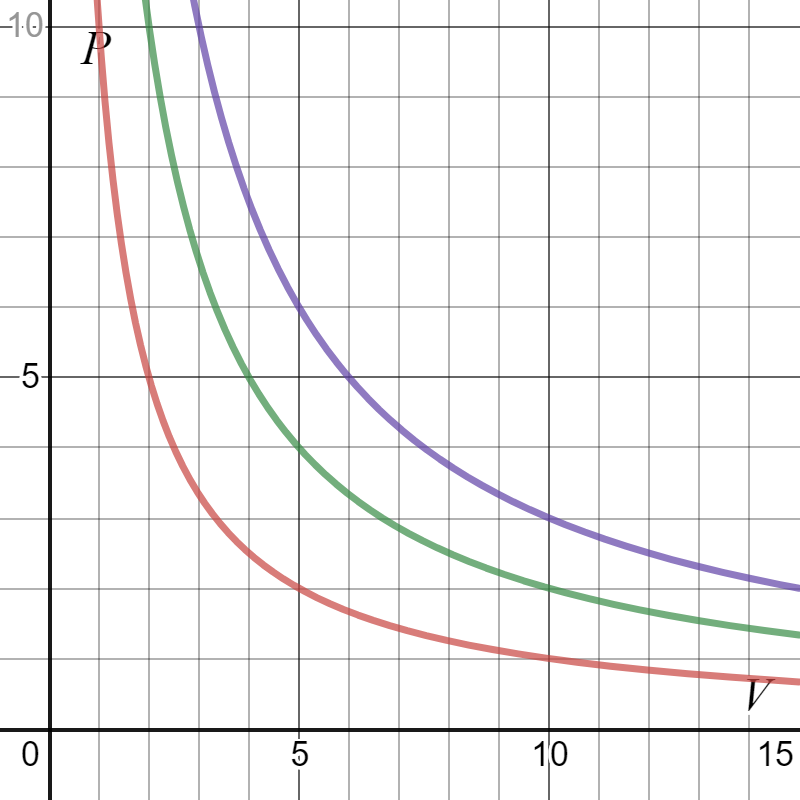
\includegraphics[width=0.5\textwidth]{isotermas.png}
    \caption{Gráficos de $PxV$ para várias $P(V)$ com $T$ diferentes. A curva em azul possui um $T$ (temperatura) do que a curva em verde e a curva em vermelho.}
    \label{fig:isoterma}
\end{figure}

\subsection{Transformações Isocóricas (Isovolumétricas)}

Essa classe de transformação ocorre quando: $\mathbf{V_i = V_f = V}$. Então, nós podemos cancelar os volumes da Equação de Clayperon e obtemos:

\begin{equation}
    \frac{P_i}{T_i} = \frac{P_f}{T_f} = \text{constante}
\end{equation}

\textbf{Para essa equação, damos o nome de Lei de Gay-Lussac.}

Essa transformação ocorre quando aquecemos uma garrafa rígida com um gás dentro. Como o volume não aumenta, a pressão e a temperatura aumentam de forma que $P/V$ é um valor fixo.

\subsection{Transformações Isobáricas}

Essa classe de transformações são para: $\mathbf{P_i = P_f = P}$. Então, da equação de Clapeyron, podemos cancelar os termos da pressão, resultando:
\begin{equation}
    \frac{V_i}{T_i} = \frac{V_f}{T_f} = \text{constante}
\end{equation}

\textbf{Essa equação damos o nome de Lei de Boyle.}

Um exemplo de transformação desse tipo é quando se aquece um gás dentro de uma seringa com êmbolo móvel. Conforme o gás aumenta a temperatura, ele pressiona o êmbolo, aumentando o volume também.

\section{Exemplos}

\begin{enumerate}
    \item 
\end{enumerate}
\end{document}
